% Attention:
% 1. Please use the XeLaTex compiler, otherwise there will be some problems with chinese compilation.
% 2. The entire document use the Mircosoft YaHei, please ensure you have installed it. Or you can substitute the fonts.
\documentclass{beamer}%[hyperref,UTF8,11pt]
\usepackage{ctex}
\usepackage[utf8]{inputenc}
\setbeamersize{text margin left=0.042\paperwidth,text margin right=0.042\paperwidth} % Adjust the left and right margins.

\usepackage{fontspec}
\usepackage{comment}
\usepackage{xeCJK}
\usepackage{hyperref}
\usepackage{graphicx}
\usepackage{epstopdf}
\usepackage{bm}

\usepackage{caption}
\captionsetup{font={scriptsize}}

\usepackage{array} 
\usepackage{cases}
\usepackage{multirow} 
\usepackage{enumerate}
\usepackage{algorithm}
\usepackage{algorithmic}
\usepackage{xcolor}
\usepackage{amsmath, amsfonts, amssymb} % math equations, symbols
\usepackage[english]{babel}
\usepackage{color}      % color content
\usepackage{graphicx}   % import figures
\usepackage{url}        % hyperlinks
\usepackage{bm}         % bold type for equations
\usepackage{multirow}
\usepackage{booktabs}
\usepackage{epstopdf}
\usepackage{epsfig}
\usepackage{algorithm}
\usepackage{algorithmic}
\hypersetup{CJKbookmarks=true}
\usepackage{url}
\usepackage{amsmath}
\usepackage{amsthm}
\newtheorem{assumption}{假设}
\newtheorem{proposition}{性质}
\usepackage{booktabs} 

\usepackage[backend=bibtex,style=numeric,sorting=none]{biblatex}
\addbibresource{reference.bib} % introduce the reference file.
\setbeamerfont{footnote}{size=\tiny}

\setcounter{tocdepth}{1}
\usepackage{subcaption}
\usepackage{amsmath}

\usepackage{sdubeamer}
\graphicspath{{image/}}

\setsansfont{Microsoft YaHei} % You can change the fonts if your computer don't have the corresponding font.
\setCJKmainfont{SimSun}
%\setCJKmainfont{SimHei}
\usefonttheme{professionalfonts}



% the settings of first page.
\title[beamer template]{\zihao{5} Title example} % [footer] {First page title}

\subtitle{\quad\quad\quad\quad\quad—————subtitle here}


\author{\noindent your name}
\institute[SDU]
{   
	\noindent your institute\\
	\medskip
	\noindent \textit{ youremail@example.com} 
}
\date{\noindent 20xx年x月x日}

\AtBeginSection[]% Add a contents page before every section.
{
	\begin{frame}{Contents}
		\transfade % fade in and out effect
		\tableofcontents[sectionstyle=show/shaded,subsectionstyle=show/shaded/hide] % Highlighte current section, dilute other sections.
		\addtocounter{framenumber}{-1}  % the contents pages do not count in total page.
	\end{frame}
}


\begin{document}
\begin{frame}
	\pgfdeclareimage[width=\paperwidth,height=0.9575\paperheight]{bg}{}
	%\transfade % fade in fade out.
	\titlepage % Print the title page as the first slide
\end{frame}

%\section{You can add section}
\begin{frame}
	\frametitle{Paper Introduction Example}
	
	\begin{columns}[T] % align columns
		\begin{column}<0->{.40\textwidth}
			\begin{figure}[htpb]
				\centering
				\resizebox{1\linewidth}{!}{
					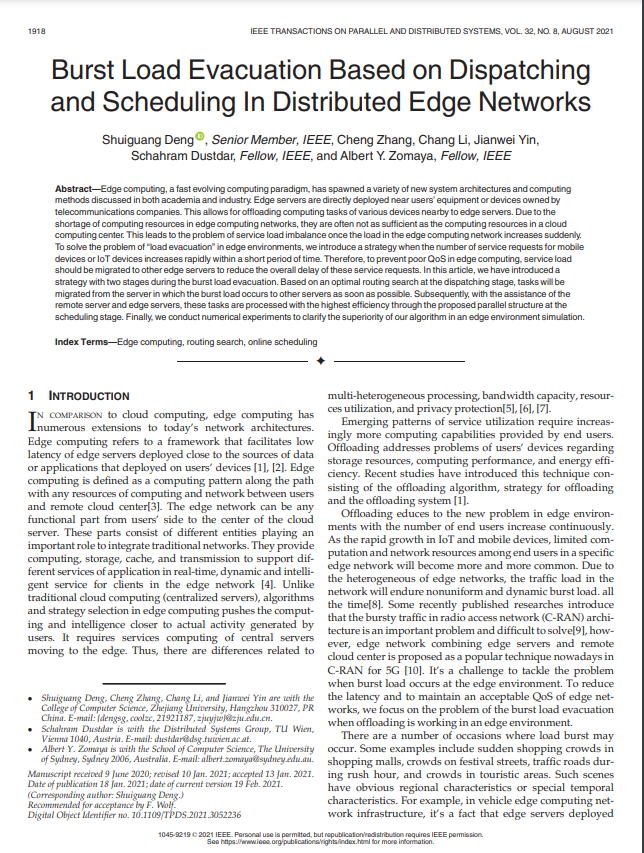
\includegraphics[scale=1.0]{paper.png}
				}
				\label{fig:paper}
			\end{figure}
		\end{column}%
		
		\hfill%	
		\begin{column}<0->{.65\textwidth}
			\begin{itemize}
				\item<1-> S. Deng, C. Zhang, C. Li, J. Yin, S. Dustdar and A. Y. Zomaya, "Burst Load Evacuation Based on Dispatching and Scheduling In Distributed Edge Networks," in \emph{IEEE Transactions on Parallel and Distributed Systems}, vol. 32, no. 8, pp. 1918-1932, 1 Aug. 2021, doi: 10.1109/TPDS.2021.3052236.
				\item<1-> Innovations
				      \begin{itemize}
					      \item<1->point one
					      \item<1->point two
				      \end{itemize}
			\end{itemize}
		\end{column}%			
	\end{columns}
\end{frame}





\begin{frame}{Contents}  % the contents of this slides, which can be commented out.
	%\transfade %fade in and out 
	\tableofcontents 
\end{frame}


\section{Text section}

\begin{frame}
	\frametitle{The reference exmaple}
	\begin{itemize}
		\item<1-> The reference are used as follows:
		      \begin{itemize}
			      \item<1->In the article\footfullcite{8549396} , the author proposed a new algorithm.
			      \item<1->In order to do something,article\footfullcite{6655873}designed the example protocol.
			      \item<1->Someone\footfullcite{7307234} used the example algorithm to address the problem.
		      \end{itemize}
	\end{itemize}
\end{frame}

\begin{frame}
	\frametitle{The example of formula reference}
	\begin{itemize}			
		\item<1->The reference of formula is as follows:
		      \begin{itemize}
			      \item<1->$x={r_1,r_2,…,r_N}$, find the optimal solution:
			      \item<1->thus the $P2$:
			            \begin{align*} \mathcal {P}_2: & \min \limits _{x \in \mathcal {X}} \max ({r_1, \ldots, r_N}) \tag{8}
			            \end{align*}
			            
		      \end{itemize}
		\item<1->this is a random sentence:
		      \begin{itemize}
			      \item<1->$H={h:X→Q}$,where $Q$ is the optimal solutions.
			      \item<1->$S_0={(x_0,y_0),…,(x_U,y_U)},$
		      \end{itemize}
	\end{itemize}
\end{frame}


\section{Image section}

\begin{frame}
	\frametitle{The example of mixed text and image}
	
	\begin{columns}[T] % align columns
		\begin{column}<0->{.65\textwidth}
			\begin{itemize}
				\item<1-> Item1
				      \begin{itemize}
					      \item<1->Item1.1 This is a randomly generated sentence
					      \item<1->Item1.2 This is a randomly generated sentence
					      \item<1->Item1.3 This is a randomly generated sentence
				      \end{itemize}
				\item<1-> Item2
			\end{itemize}
		\end{column}%			
		\hfill%	
		\begin{column}<0->{.40\textwidth}
			\begin{figure}[htpb]
				\centering
				\resizebox{1\linewidth}{!}{
					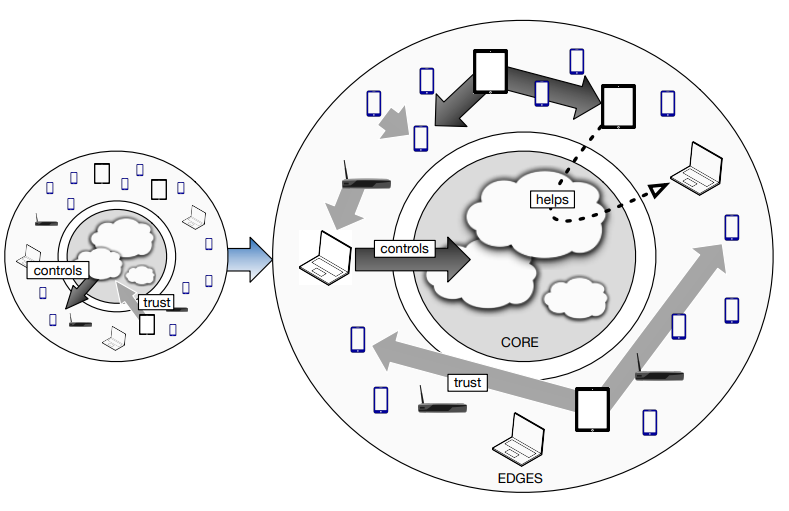
\includegraphics[scale=1.0]{edge.png}
				}
				\caption{Centralized cloud model (left) versus
					Edge-centric Computing (right).}
				\label{fig:edge}
			\end{figure}
		\end{column}%
	\end{columns}
\end{frame}


\begin{frame}{The example of combining formula and image}
	\begin{columns}[T] % align columns
		\begin{column}<0->{.65\textwidth}
			\begin{itemize}
				\item<1-> index set of tasks as $\mathcal{N} \triangleq\{1,2, \ldots, N\}$
				\item<1->the index set of edge servers as $\mathcal{M} \triangleq\{1,2, \ldots, M\}$
				\item<1->We denote the indicator of a task latency in burst load as $I^{\dagger }_i(t)$.While $I^{\dagger }_i(t) = 1$  means waiting.
				      
				      \begin{itemize}
					      \item<1->The latency time of the ith task denoted as:
					            \begin{equation*} T_1^i = \sum _{t>0} I^{\dagger }_i(t), \tag{1}
					            \end{equation*}
				      \end{itemize}
			\end{itemize}
		\end{column}%			
		\hfill%	
		\begin{column}<0->{.40\textwidth}
			\begin{figure}[thpb]
				\centering
				\resizebox{1\linewidth}{!}{
					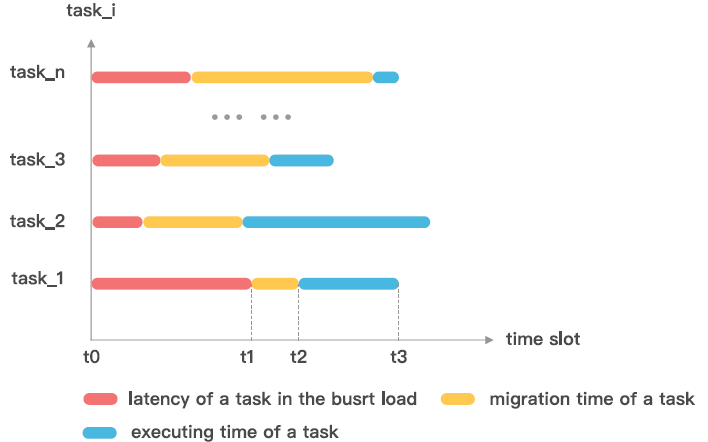
\includegraphics{tasks.png}
				}
				%\includegraphics[scale=1.0]{figurefile}
				\caption{The flowchart of tasks when evacuation}
				\label{fig:tasks}
			\end{figure}
		\end{column}%
	\end{columns}
\end{frame}




\begin{frame}{The example of two images}
	\begin{figure}[htb]
		%  \centering
		\label{fig:example}
		\begin{subfigure}{.45\textwidth}
			\centering
			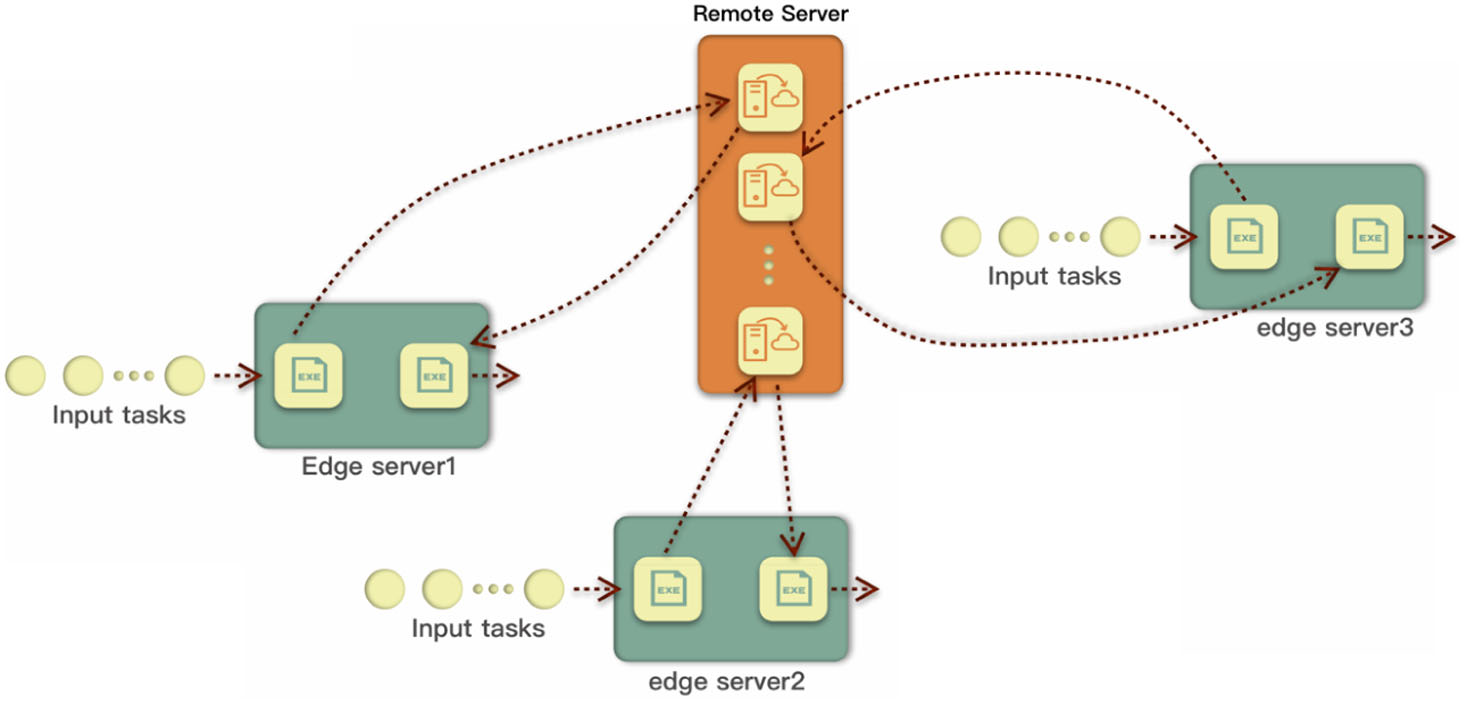
\includegraphics[width=\textwidth]{scheduling.jpg}
			\caption{Task scheduling for executing and requesting data}
			\label{fig:scheduling}
		\end{subfigure}
		\begin{subfigure}{.45\textwidth}
			\centering
			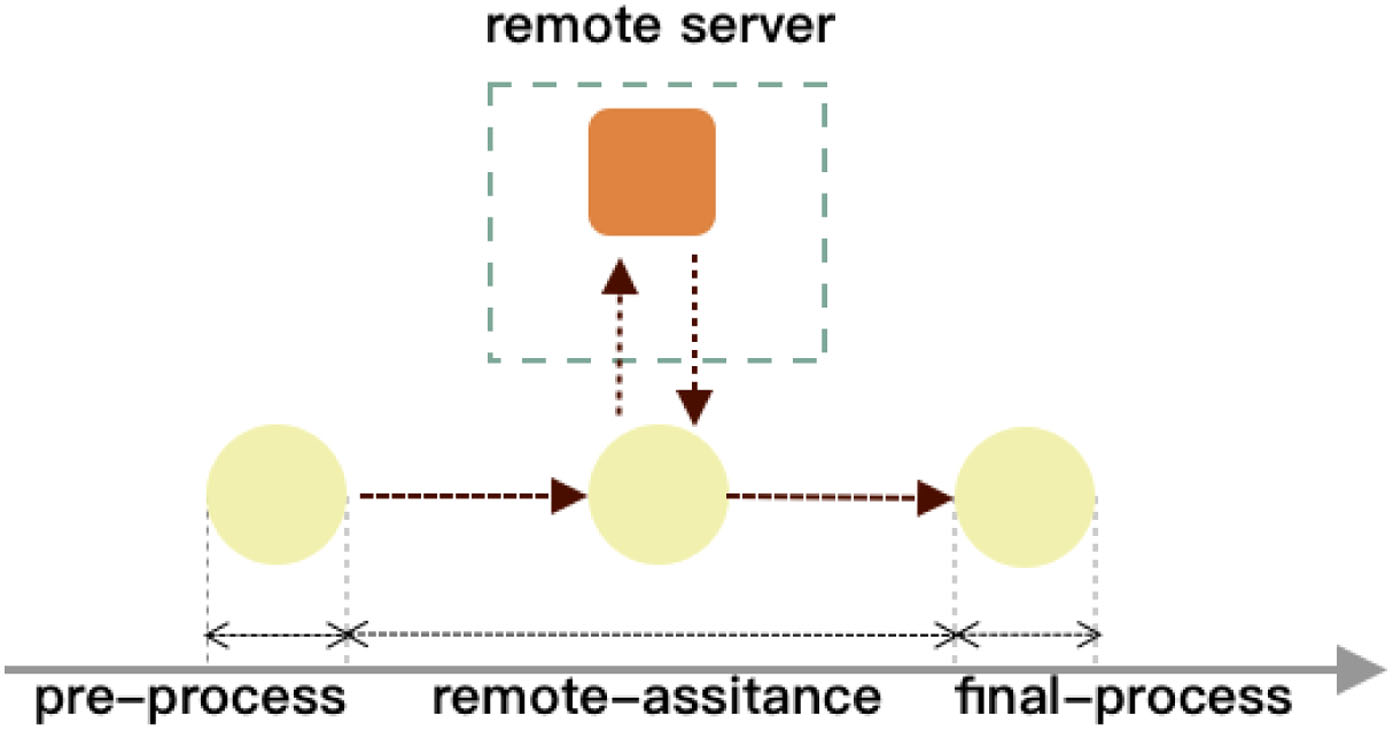
\includegraphics[width=\textwidth]{processing.jpg}
			\caption{Task processing sequence.}
			\label{fig:logob}
		\end{subfigure}
		%\note{note:}
	\end{figure}
\end{frame}


\begin{frame}
	\frametitle{The example of single image}
	
	
	\begin{figure}[htpb]
		\centering
		{
			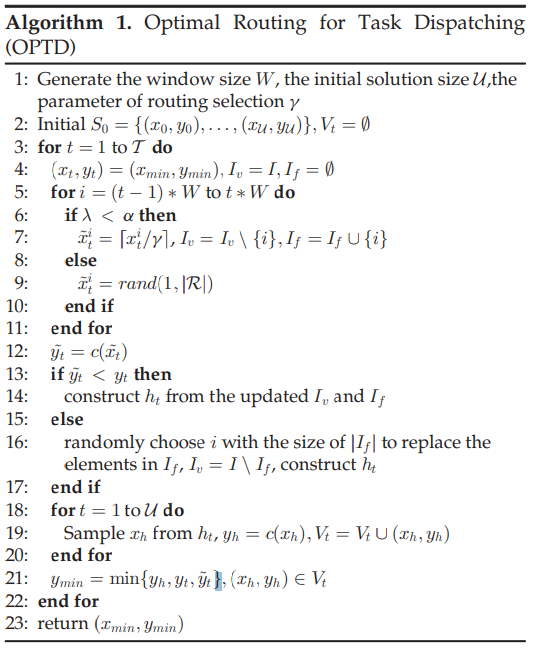
\includegraphics[scale=0.3]{algorithm1.png}
		}
		\label{fig:algorithm1}
	\end{figure}
	
	
\end{frame}


\begin{frame}
	\frametitle{Reference}
	\printbibliography
\end{frame}


\begin{frame}
	\frametitle{Acknowledgement}
	\begin{itemize}

		\item<1->thank y'all.
		      
	\end{itemize}
\end{frame}
\end{document}